% Local build wrapper (not needed on Overleaf, where main.tex compiles directly).
%
% Some TeX installations ship a `figureversions` package (loaded by acmart's fonts)
% that is newer than their LaTeX kernel and calls an expl3 function the kernel
% does not have yet. The function is defined here if it is missing, so that
% main.tex stays exactly as the organisers' template expects it.
%
%   pdflatex -jobname=main build_local.tex && bibtex main
%   pdflatex -jobname=main build_local.tex && pdflatex -jobname=main build_local.tex
\ExplSyntaxOn
\cs_if_exist:NF \prop_gput_if_not_in:Nnn
  {
    \cs_new_protected:Npn \prop_gput_if_not_in:Nnn #1#2#3
      { \prop_if_in:NnF #1 {#2} { \prop_gput:Nnn #1 {#2} {#3} } }
    \cs_generate_variant:Nn \prop_gput_if_not_in:Nnn { NnV , Nnv , NVn , NVV , cnn , cnV }
  }
\cs_if_exist:NF \prop_put_if_not_in:Nnn
  {
    \cs_new_protected:Npn \prop_put_if_not_in:Nnn #1#2#3
      { \prop_if_in:NnF #1 {#2} { \prop_put:Nnn #1 {#2} {#3} } }
    \cs_generate_variant:Nn \prop_put_if_not_in:Nnn { NnV , NVn , NVV , cnn , cnV }
  }
\ExplSyntaxOff
\documentclass[sigconf,nonacm]{acmart}
\title{Bidirectional Window Matching for Multimodal Human Activity Recognition on WEAR}
\author{Gaurav Vyas}
\hypersetup{colorlinks=true,linkcolor=blue,citecolor=blue,urlcolor=blue}
\begin{abstract}
Recognizing outdoor exercise activities from shuffled one-second windows is difficult when different movements share similar poses. We present the solution submitted by Gaurav Vyas to the 3rd WEAR Dataset Challenge at HASCA 2026. A multimodal ensemble combines inertial measurements and egocentric VideoMAEv2 features. Independent successor and predecessor rankers build a participant-specific graph for refining activity predictions. The selected submission scored 0.93821 public macro-F1, compared with 0.93611 for the parent ensemble, and placed third in the final Kaggle standings as reported by the entrant. The source-side graph benchmark reached 0.93130 macro-F1.
\end{abstract}
\keywords{human activity recognition, wearable sensing, egocentric video, learning to rank, graph propagation}
\begin{document}
\maketitle

\section{Introduction}
A single second may capture a similar pose or motion phase in several activities. Although the test windows are shuffled, their observed signals can provide evidence that some windows are temporally adjacent or belong to the same exercise bout. We use that evidence to refine multimodal activity predictions. The main contribution is to rank candidate successors and predecessors independently and to enforce one-to-one assignments before propagating activity probabilities.

% Pipeline overview and measured results are included as raster figures.


\section{Data and Evaluation}
The WEAR dataset contains outdoor recordings from 22 source participants and defines 18 exercise labels and one null label \cite{wear}. The challenge test set has 12,234 windows from four additional participants \cite{challenge}. Each one-second window contains 50 triaxial acceleration samples from one sensor location and 15 supplied 768-dimensional VideoMAEv2-Base feature vectors. Participant and sensor identifiers are available. Graphs are built separately for each participant using unlabeled observations. Target labels, timestamps and true ordering are excluded from graph construction.

The official metric is macro-F1 across the 19 classes. We used five participant-grouped source folds for graph development and also computed a diagnostic on source participants with IDs of at least 14. The paired graph experiments inherit upstream stacking and activity evidence. Their scores measure relative changes under this benchmark and do not constitute a fully nested estimate of the deployed ensemble.

\begin{figure}[t]
\centering
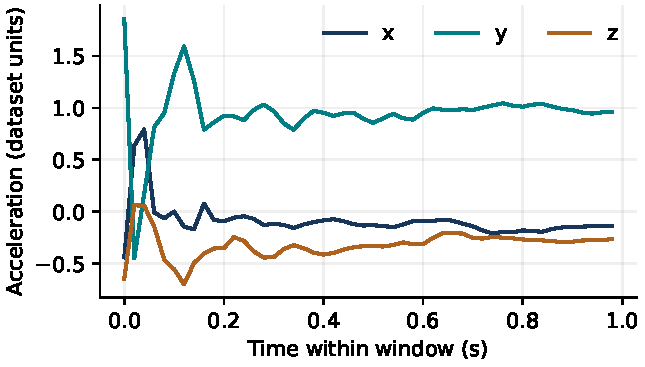
\includegraphics[width=\columnwidth]{figures/inertial_window.pdf}
\caption{Measured acceleration across three axes for one supplied test window.}
\label{fig:window}
\end{figure}

\section{Method}
\begin{figure}[tb]
\centering
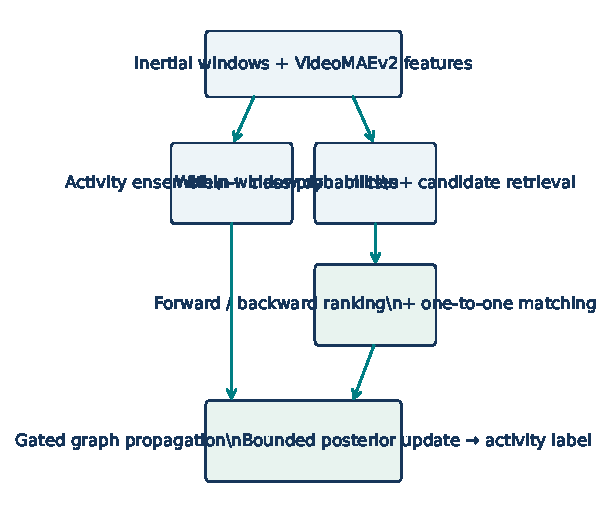
\includegraphics[width=\columnwidth]{figures/pipeline.pdf}
\caption{Two branches produce activity probabilities and a participant-specific graph. The bounded update transfers the graph's effect onto the ensemble.}
\label{fig:pipeline}
\end{figure}
Figure~\ref{fig:pipeline} summarizes the inference pipeline. The measured input in Figure~\ref{fig:window} illustrates the inertial branch.
\subsection{Multimodal activity ensemble}
The parent ensemble averages two branches with equal weights. The fold-matched branch uses neural activity evidence, self-training on unlabeled windows, and a LightGBM multiclass refiner that includes graph and chain summaries of nearby activity predictions. Two self-training runs per fold are decoded separately before averaging the ten posteriors. The second branch uses final models trained with all source participants and a chain-based activity refiner. The resulting ensemble serves as the fixed prediction base for subsequent graph changes.

\subsection{Motion features and directional ranking}
Within each participant, video frame embeddings are projected to 128 principal components. Forward and reverse ridge forecasts fitted to within-window motion extrapolate beyond the observed endpoints and retrieve additional candidate pairs. Pair features describe endpoint compatibility, graph topology, reach over up to eight graph steps, and local forecast corrections from nearby poses. The intermediate graph averages the reach-based and local-motion successor and same-bout scores while retaining the same-label channel.

The final LightGBM LambdaRank models use 120 features per pair, comprising 115 reach and context features and five local residual features. The forward ranker groups candidates by origin window, while the backward ranker groups them by destination window. The predecessor model uses 300 boosting rounds. Explicitly supplied source successor links are masked from link evaluation. At inference, query-normalized scores feed separate one-to-one assignments in each direction, using a 0.02 threshold.

\subsection{Graph decoding}
The edge score combines the learned same-bout score and same-label score with weights of 2 each and the forward and backward matched-edge channels with weights of 2.5 each. This preserves soft links when exact temporal adjacency is uncertain. We gate the edge score by \(0.25+0.75a_{ij}\), where \(a_{ij}\) is the activity-posterior affinity, then use the original decoder with top-ten neighbors, squared and symmetrized weights, 15 propagation steps, and a propagation coefficient of 0.9. The decoder retains participant-level non-null priors.

\subsection{Bounded transfer to the ensemble}
Let \(Q_{0,f}, Q_{m,f}, Q_{b,f}\) denote fold-\(f\) posteriors decoded from the original, intermediate motion, and final bidirectional graphs using identical activity evidence. Define \(D(X,Y)=\mathrm{clip}(\log X-\log Y,-2,2)\), with posterior probabilities floored at \(10^{-7}\). We update the log scores of the already motion-corrected parent prediction by
\[
\frac{1}{5}\sum_f
  [D(Q_{b,f},Q_{0,f})-D(Q_{m,f},Q_{0,f})].
\]
The subtraction prevents double counting the intermediate motion correction. The largest adjusted score determines the submitted label.

\section{Results}
\begin{table}[t]
\caption{Participant-grouped source graph benchmark and public Kaggle macro-F1.}
\label{tab:results}
\begin{tabular}{lrr}
\toprule
Configuration & Source & Public\\
\midrule
Parent ensemble (c102) & 0.92988 & 0.93611\\
Motion graph (c129) & 0.93041 & 0.93733\\
One-to-one motion match (c157) & 0.93067 & 0.93748\\
Forward ranker (c164) & 0.93092 & 0.93744\\
Forward matched core (c172) & 0.93109 & 0.93773\\
Bidirectional matched core (c173) & \textbf{0.93130} & \textbf{0.93821}\\
\bottomrule
\end{tabular}
\end{table}

The final graph improved public macro-F1 by 0.00210 over the parent ensemble (Table~\ref{tab:results}). Relative to the forward rank reference, the source result improved in four of five folds, correcting 87 errors and introducing 63 new errors. Source macro-F1 for participants with IDs of at least 14 was 0.95595. Predecessor precision increased from 0.67348 to 0.69920 on the source link benchmark. The final graph changed 33 test predictions relative to the intermediate motion graph. Directly re-decoding the individual members with the final graph scored 0.93810 on the public leaderboard.

The selected Kaggle file was \texttt{c173\_bidir\_consensus\_core.csv}, submission reference 57113473, under the display name Gaurav Vyas. The entrant reports a final Kaggle rank of 3. The final private macro-F1 is pending verification.

\begin{figure}[t]
\centering
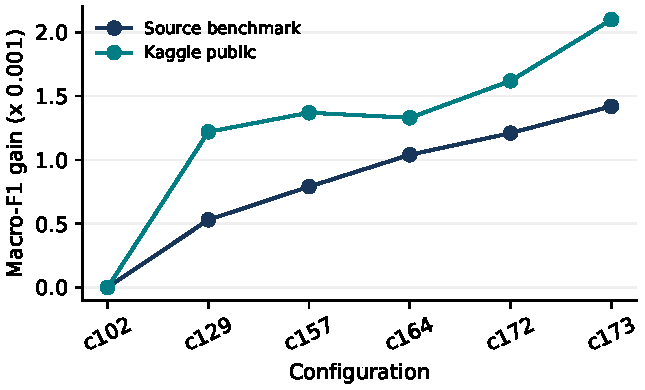
\includegraphics[width=\columnwidth]{figures/benchmark.pdf}
\caption{Macro-F1 gain relative to the parent ensemble, shown separately for the source benchmark and public leaderboard.}
\label{fig:scores}
\end{figure}

\section{Data and Code Availability}
The \href{https://www.kaggle.com/competitions/3rd-wear-dataset-challenge-hasca-2026/data}{Kaggle data page} provides the accelerometer windows, video features, metadata, and label mapping. The accompanying repository contains the exact submitted predictions, benchmark scores, figure-generation code, and the matching implementation. The \href{https://www.kaggle.com/competitions/3rd-wear-dataset-challenge-hasca-2026/leaderboard}{Kaggle leaderboard} lists competition results. See Figure~\ref{fig:scores} for the measured changes across configurations.

\section{Limitations and Conclusion}
The solution uses unlabeled windows from the same participant at inference, so its results describe batch prediction. Repeated movements can create plausible but incorrect matches, and missing intermediate windows limit the recoverable temporal structure. The four test participants and the development use of public leaderboard feedback limit the scope of generalization claims. Within the recorded development comparisons, bidirectional matching improved the graph refinement while preserving the underlying multimodal ensemble.

\begin{thebibliography}{2}
\bibitem{wear} Marius Bock et al. WEAR: An Outdoor Sports Dataset for Wearable and Egocentric Activity Recognition. arXiv:2304.05088. \url{https://arxiv.org/abs/2304.05088}
\bibitem{challenge} Marius Bock et al. 2026. 3rd WEAR Dataset Challenge. \url{https://mariusbock.github.io/wear/challenge.html}
\end{thebibliography}
\end{document}

